\chapter{Implementation}

	\section{Dictionary of Songs}
		The Trie (Section \ref{sec:trie}) data structure is used to load the Million Song Dataset (Section \ref{sec:million_song_dataset}). Trie enables faster searching and computation of Levenshtein Distances (Section \ref{sec:levenshtein_distance}) for the titles of the songs. The titles of the songs are used as an index for the \emph{trie}. Each node of the \emph{trie} stores with itself some data which is used frequently, for example, its unique track ID using which all other song informations can be referenced from the MIllion Song Dataset and artist information. We store the artist, as a song is uniquely identified by its title and artist, which is used for other API calls in the subsequent steps. The \(999,999\) songs from the dataset occupies \(6,510,645\) nodes.
	
	\section{User History}
		A set of \(2614\) users a with considerable amount of playback history has been compiled. These users' histories will serve as the basis for obtaining recommendations from similar users using \emph{collaborative filtering}. The limit on the number of recent tracks taken per user is \(200\). This gives us a considerable number of tracks to perform analysis upon.
		
		Each track is cross-referenced with those in the MIllion Song Dataset by searching within the above discussed \emph{trie}. Only those tracks which find a match are kept and the others are discarded. However, the track names scrobbled by Last.fm are often custom written by 3\textsuperscript{rd} party and/or the users themselves, in which case even a slight change in the name will deem it to be discarded. \emph{Levenshtein Distance} has been used to match each of the fetched song. A threshold distance of \(2\) gives the optimal number of track filtering. Anything lesser would make the filter too strict thus losing too much of valuable user history; whereas keeping it higher will corrupt the data with too many incorrect matches.
		
		A few other information available with the \emph{Million Song Dataset}, for example, \emph{loudness}, \emph{tempo}, \emph{hotness} are also loaded into memory at this step. This is a part of pre-processing of the data and would considerably lower the runtime of generating the recommendations. These features has been described below in Section \ref{sec:recommend}.
	
	\section{Model User Interests}
		A set of \(127\) commonly recognized genres (often referred to as track tags) has been compiled. Each song is classified in one or more of these genres. These genres compiled for a given set of tracks will dictate the musical taste of a user. This goes forward to define the user's music preferences. The genres of each song uniquely identifed by its \emph{title} and \emph{artist name} from the user's history is fetched and added to the pool of genres.
		
		The pooled genres for a user is represented using a vector of integers, each representing the total count of the respective genre in her given music history.
	
	\section{Determine Similar Users}
		The similarity between users are determined by their music preferences determined by the pool of genres obtained from each of the songs from their respective music histories. The similarity between user \(X\) and user \(Y\) is calculated on their respective vectors as follows.
		
		\[ similarity (X, Y) = \sum_{i} min(X_i, Y_i) - |X_i - Y_i| \]
		
		Using \(kNN\) with \(k = 200\), the top \(k\) similar users have been chosen. These users' histories will be searched and used to recommend songs for any given user. 
	
	
	\section{Recommend Songs}
	\label{sec:recommend}
		\subsection{Defining Mood}
			Assuming an average song has a runtime duration of \(3 minutes\), the mood of a user is determined by the latest \(10\) songs from her history, i.e., 30 minutes. It is assumed that the mood of a user changes gradually with time and the songs she listens and is considerably constant over the period the \(10\) songs. Thus, a rolling window of latest songs is used at any point of time.
			
		\subsection{Collaborative Filtering}
			The mood of the current user, i.e., the recent \(10\) songs, is compared to other rolling windows in the histories of the ``similar'' users. The rolling window in the ``similar'' user's history can be in any order, but necessarily consecutive. The track listened to by the ``similar'' user just after the rolling window in consideration, is taken as the recommendation for that window. So, every window has a recommendation with the similarity to the given user's mood as its confidence score. These recommendations for each window for each of the ``similar'' users are then sorted and the best \(5\) recommendations are presented to the given user.
			
			The similarity between the windows of the given user and a similar user is determined by the use of the \emph{Hungarian Algorithm} (Section \ref{sec:hungarian}). The cost matrix used by the algorithm is generated by calculating the similarities (subsection \ref{subsec:song_similarity}) between each pair of songs, \(1\) from each of the windows. The algorithm is applied on the thus formed \(10\) x \(10\) matrix.
			
		\subsection{Song Similarity}
		\label{subsec:song_similarity}
			The following parameters define certain properties of a song.
\begin{itemize}
	\item Loudness: Overall song loudness is a formula combining segments: local maximum loudness, dynamic range, overall top loudness, and segment rate. The greater the dynamic range, the more influential it is on lowering the overall loudness. The loudness reference is currently -60dB.
	\item Tempo: The average beats per minute of a song contributes to the tempo. This determines the pace of the song, for example, if the song is a slow one or a fast.
	\item Hotness: This is a measure of the popularity of the song among users. It plays a significant role in the recommendation as users might want to hear new and top of the chart songs even if it does not flare well according to her mood.
\end{itemize}

			Over and above these parameters, the comparing the artist is crucial, as more often than not, users choose to remain loyal to a certain set of artists. The Million Song Dataset happens to provide us with a vector of genres for each artist. The cosine similarity (Section \ref{sec:cosine_similarity}) is used to compare the genre vectors of the artists for a given pair of songs.
			
			These \(4\) parameters contribute to the determination of the similarity between a pair of songs. A weight of \(0.25\) has been provided to each as they are equally significant towards recommendation.

	\section{Work Flow Summary}
		\begin{figure}[h!]
			\centering
			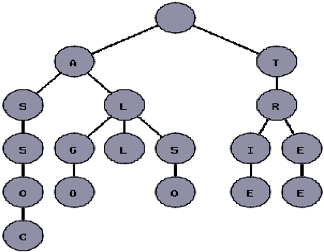
\includegraphics[width=15cm]{trie.png}
			\caption{Work Flow}
		\end{figure}
			